\documentclass[11pt]{article}
\usepackage{amssymb}
\usepackage{algpseudocode}
\usepackage{algorithm}
\usepackage{setspace}
\usepackage{graphicx}
\graphicspath{ {./images/} }
\usepackage{hyperref}
\usepackage{siunitx}

\hypersetup{
    colorlinks=true,
    linkcolor=blue,
    filecolor=magenta,      
    urlcolor=cyan,
}

\title{MSc Project - Binding Affinity Prediction of Protein-Ligand Complex}
\author{
        Abdus Salam Khazi\\
        \href{mailto:abdus.khazi@students.uni-freiburg.de}
                {abdus.khazi@students.uni-freiburg.de}\\ \\
        \href{https://github.com/abduskhazi/MSc-Project}
                {Github Repository} \cite{github_repository} \\ \\
        Supervisors:
        \begin{tabular}{ll}
			Simon Bray \&
			Alireza Khanteymoori
		\end{tabular}
       }
	
\begin{document}

\maketitle
\date{}
\tableofcontents
\newpage

\section{Introduction}
.....TOBE REFINED AFTER COMPLETING THE FULL REPORT.....

\subsection{Biological Background}
Proteins are the workhorses of our body.
Every main function is carried out by a protein or a collection of proteins.
Ligands are molecules that bind to proteins to form protein-ligand complexes.
They can be molecules that the protein transports e.g. Haemoglobin transporter
or they can act as stimulating agents.
In addition to this, they can also start/stop the protein from doing its function.
The correct functioning of these protein-ligand complexes is essential for any living organism.

The study of protein-ligand complexes is an intrinsic part of the drug discovery field.
This is because drugs are small molecules that act as ligands.
As the drug molecules (ligands) bind to the target proteins, they can artificially influence
the protein behavior which causes a therapeutic effect.

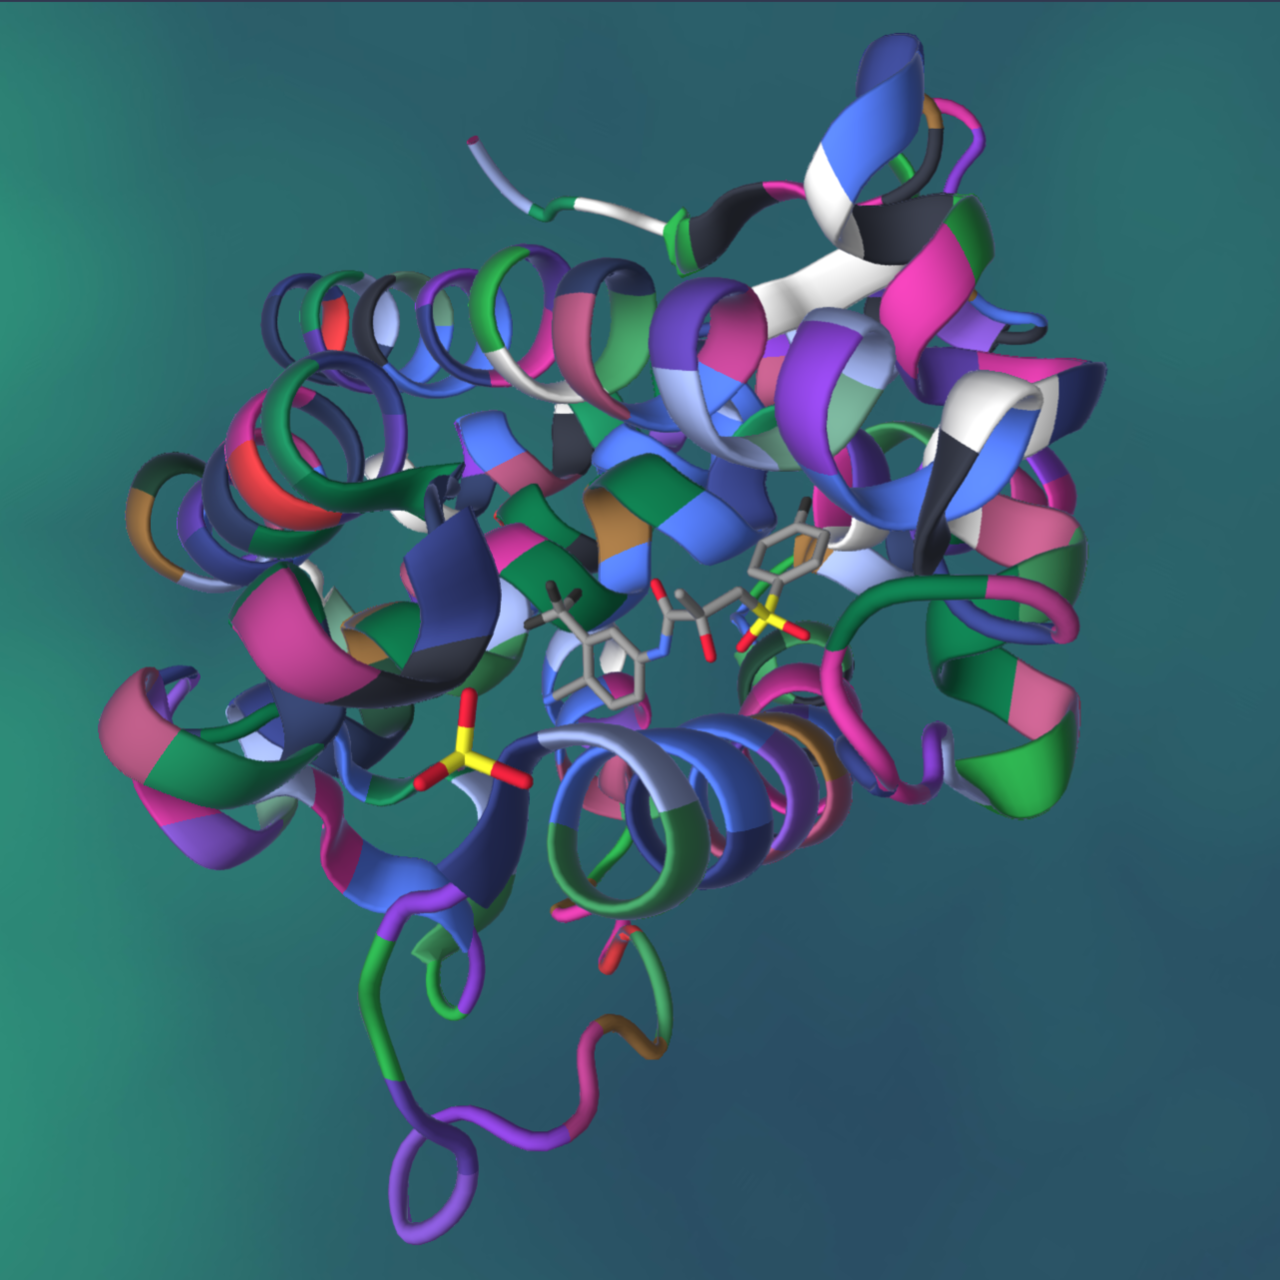
\includegraphics[scale=0.15]{pl_complex}
\cite{PL_complex_introduction}

When one proposes a target drug candidate, he has to answer questions
like - How easily does the drug bind to the target protein?
Does it bind to any other protein - If so is it desirable?
Does it have any unforeseen effect on the protein function?
etc.
To answer these questions biologists and pharmacists conduct wet-lab experiments which are expensive.

One way to reduce the cost of these experiments is to make a data-driven selection of the drugs.
Using experimental data collected over many years, one can build models to predict the
behavior of the proposed drug computationally.
These 'In-Silico' computational methods can aid in the elimination of undesirable drugs as well guide the drug selection process.

Our project aims to answer one of the above questions - How well does a given drug bind to the target protein?
We determine this computationally by building a machine learning model that is trained on the previous data.
We hope that this model will be helpful in reducing the costs of drug discovery.
But from where do we get the data to build our model?

\subsection{PDBBind Dataset}
Over the last few decades, researchers have been successful in building a single data archive for proteins.
This archive, called \textbf{Protein Data bank} \cite{pdb_homepage} , holds 3-D structural data of the proteins determined by experiments
like X-ray crystallographic, Nuclear magnetic resonance (NMR), and cryoelectron microscopy (cryoEM).
A subset of this data also contains information about how well a given protein and ligand bind together.
It is called binding affinity between a protein and ligands.
(It also contains data about protein-protein complexes which isn't dealt with in our project)
\cite{pdbank_history}

As we are studying the protein-ligand binding affinity, we would like to filter out this data from the protein data bank.
It is what is done by the maintainers of the \textbf{PDBBind Data bank}.
\cite{pdbbind_introduction}
Using the curated protein-ligand affinity data present in the PDBBind Data bank, we build a machine learning model that learns to predict the affinity.
But how is the binding affinity quantified?

\subsection{Understanding Binding Affinity}
A binding affinity between a protein and a ligand is quantified by the $K_d$, $K_i$ and $IC_{50}$ measures in the PDBBind Data bank.
Here $K_d$ refers to disassociation constant, $K_i$ refers to the inhibition constant and $IC_{50}$ refers to 
inhibitory concentration 50\%.
The reason for having different measurements is because it is not possible to use the same measurement techniques
for all biological complexes/processes.

To understand $K_d$, consider a protein and a ligand binding and unbinding continuously in a kinetic system.
In this system let $[P]$, $[L]$ and $[PL]$ represent the concentrations of the Protein, Ligands 
and the protein-ligand complex respectively.
This system can be represented by the equation.
$$[P] + [L] \rightleftharpoons [PL]$$
We can quantify the binding affinity $K_d$ by using the concentrations in the above system at equilibrium.
$$K_d = \frac{[P][L]}{[PL]} = \frac{k_{-1}}{k_1}$$
where $k_{-1}$ is the disassociation rate constant and $k_1$ is the association rate constant.
Similarly, $K_i$ and $IC_{50}$ are defined using concentration albeit non-trivially. 
\cite{binding_affinity_description}

Our problem, hence, boils down to this - Given $K_d$/$K_i$/$IC_{50}$ for various complexes in the PDBBind Data bank,
can we predict this affinity measure for new protein-ligand complexes?

The next questions that need to be answered before we build our agent are - how exactly are the proteins and ligands represented in the PDBBind Data bank?
How do we extract the properties of proteins and ligands for predicting this affinity?

\section{Problem Set-up and Formulation}

The binding of proteins and ligands is heavily influenced by their respective 3D structures.
The \textbf{PDBBind Data bank} extracts information about these complexes from the \textbf{Protein Data bank} and creates the following files for every complex
\begin{itemize}
\item \textbf{PDB Format} - For the Protein.
\item  \textbf{Mol2} - For the ligand.
\item \textbf{SDF} - For the ligand.
\end{itemize}

All of the above formats contain the 3D information that is essential in the prediction of the binding affinity.
The 3D representation of the proteins and ligands is encoded like in the \textbf{XYZ format}.

\subsection{XYZ format}

XYZ format is a chemical file format that is used to represent the geometry of a molecule.
It specifies the number of atoms and their Cartesian X, Y, Z coordinates hence the name XYZ format.
These coordinates given are relative to each other hence, translation and rotation do not change the molecule's representation. 
The following text shows the XYZ format representation and an example.
\cite{XYZ_format}

\begin{verbatim}
<number of atoms>
comment line
<element> <X> <Y> <Z>
...
\end{verbatim}

The units of distance used is Angstrom (\si{\angstrom}).  \SI{1}{\angstrom} $ = 10^{-10}$ m.
For example, the pyridine molecule is represented in the following format.
\cite{XYZ_format}

\begin{verbatim}
11

C       -0.180226841      0.360945118     -1.120304970
C       -0.180226841      1.559292118     -0.407860970
C       -0.180226841      1.503191118      0.986935030
N       -0.180226841      0.360945118      1.29018350
C       -0.180226841     -0.781300882      0.986935030
C       -0.180226841     -0.837401882     -0.407860970
H       -0.180226841      0.360945118     -2.206546970
H       -0.180226841      2.517950118     -0.917077970
H       -0.180226841      2.421289118      1.572099030
H       -0.180226841     -1.699398882      1.572099030
H       -0.180226841     -1.796059882     -0.917077970
\end{verbatim}

\subsection{PDB, SDF and Mol2 formats}

PDB format is a human readable file format used to represent the protein molecules (macro molecules).
In addition to the 3D information of atoms,
it contains information regarding protein's primary, secondary, tertiary
and the quaternary structures.
Because of the presence of 3D positional data, molecular visualization is possible using specialized software. 
\cite{pdb_file_format}
\cite{understanding_pdb_format}

SDF format file is a type of molecular descriptive file which contains x,y,z format similar to pdb format.
It also contains bond information.
This data can be used to create a graph using which SMILES string can be created.
\href{https://en.wikipedia.org/wiki/Chemical_table_file}{SDF format}

Mol2 format file is also a file similar to the sdf format.
We chose to use this format because we could extract the features of more molecules
using this format as compared to the sdf format.


\subsection{Problem Formulation}
Protein-Ligand complex problems can be broadly classified into 2 types -
\begin{itemize}
\item LBS - Ligand binding site prediction.
\item Ligand affinity prediction.
\end{itemize} 

LBS (Ligand binding side) prediction can be further classified into 3 types -
\begin{itemize}
\item 3D structure based
\item Template based
\item Sequence based
\end{itemize}

The problem that we deal is Binding affinity prediction. 
The protein ligand complex binding affinity is defined by a number Kd which is called dissociation constant.
This constant is given for all pl complexes in the pdb bind dataset.
In our problem we take care of the following 2 things
\begin{itemize}
\item We do not take the features of the whole protein
but take the features of the location of the protein which binds to the ligand.
This is called a pocket.
\item We try to keep the features of proteins and ligands distinct till the input so that we can have a plug and play sort of input for our model.
The binding affinity of any protein or ligand can be found out because of this property of our modelling.
\end{itemize}

However for this we make use of existing 3D structure based LBS tool chain called fpocket.
The reason this is helpful is because 3D structural features of proteins are very crucial for the binding between 
the proteins and ligands as proteins and ligand interactions can be considered as
machines of 2 parts interacting with each other.

\subsection{fpocket/dpocket descriptors}
We extract the features of a pocket using dpocket tool (a submodule in the fpocket toolchain).
fpocket uses veronoi tessalation (3D) to find out pockets in our protein structure.
To get the descriptors/features of the pockets at which ligands bind we use the dpocket (aka descriptors pocket).
dpocket creates 3 types of descriptors for the pockets in the protein -
\begin{itemize}
\item fpocketp.  This lists all the possible pockets (with descriptors) that could bind to ligand according to a criteria.
Multiple pockets can bind with the same ligand.
Here the descriptor called overlap maybe 100\% or less.
\item fpocketnp.  This lists all pockets (with descriptors) that are not binding according to the criteria.
\item explicitp.
This lists all the explicitly binding pocket (with descriptors).
Here the overlap feature is always 100\%.
\end{itemize}

We use both fpocketp and explicitp descriptors to train our model.
There are in total 55 descriptors in total obtained using dpocket descriptors.



\section{Feature selection}

\subsection{Dichotomous problem}
Since the protein and the ligand are equally responsible for the affinity between them, our problem (also the binding site prediction problems) can be classified as a dichotomous problem in which we need data from both
the protein and the ligand.
The data if it is complementary is better for solving the problem.
The accuracy measure of the protein LBS prediction is the same as the dichotomous problems in math.
As we are dealing with a dichotomous problem we have to select features of the protein and the ligand separately.
This helps us make our model plug and play w.r.t the proteins and ligands.
The following feature selection mechanisms were used to select features -

\begin{itemize}
\item Each feature of both protein and ligand were correlated with the output i.e the Dissociation constant.
We used both pearson and spearmann correlation to calculate this.
The assumption to be made when taking these correlations is that of monotonic increase of
the feature with respect to the output.
The features with the highest correlation were taken from both proteins and ligands as
inputs.
\item By using genetic algorithms\cite{genetic_algorithm}.
Here each feature is represented by a binary number.
1 indicating inclusion and 0 indicating exclusion from the input of our model.
A binary string of 456 binary numbers (401 for ligands + 55 for proteins) is called a chromosome.
See pseudocode below
\item Features selected by expert. Given by Simon Bray. (Yet to do)
\end{itemize}

\label{Genetic_Algo}
\begin{algorithm}
\caption{Selection of features in our model using genetic algorithm \cite{genetic_algorithm}}
\begin{algorithmic}[1]
\Procedure{GENETIC\_ALGORITHM\_BASED\_SELECTOR}{}
\State model\_type $\gets$ Linear Regression
\State $ population = \{C_1, C_2, C_3... C_n\}$ $\in$ $\mathbb{B}^{456}$ (initial chromosomes).
\State best $\gets C_1$ 
\State $i \gets 0$
\State $gen \gets$ number of generations to run.
      \For{\texttt{$i < gen$}}
          \State Fit model\_type for each feature selection (chromosome). 
          \State Let $\{S_1, S_2, S_3... S_n\}$ $\in$ $\mathbb{R}$ be scores for each chromosome.
          \State best $\gets$ $C_i$ with the highest score $S_i$
          \For{\texttt{$j < len(population)$}}
              \State Set $\gets$ 3 random chromosomes from $population$
              \State $c \gets best($Set$)$
              \State $genetically\_better\_population.add(c)$
          \EndFor
          \State $population \gets genetically\_better\_population$
          \For{\texttt{$j < len(population)$ with step 2}}
              \State $P_1, P_2$ $\gets$ $population[j], population[j+1]$
              \State $c_1, c_2 \gets crossover(P_1, P_2)$
              \State $c_1 \gets mutation(c_1)$
              \State $c_2 \gets mutation(c_2)$
              \State $children.add(c_1, c_2)$
          \EndFor
      \State $new\_population \gets population$
      \EndFor
\State return best
\EndProcedure
\end{algorithmic}
\end{algorithm}


\section{Discussion}


\section{Conclusion}

\bibliographystyle{plain}
\bibliography{references}

\end{document}
